\begin{figure}[t]
\centering
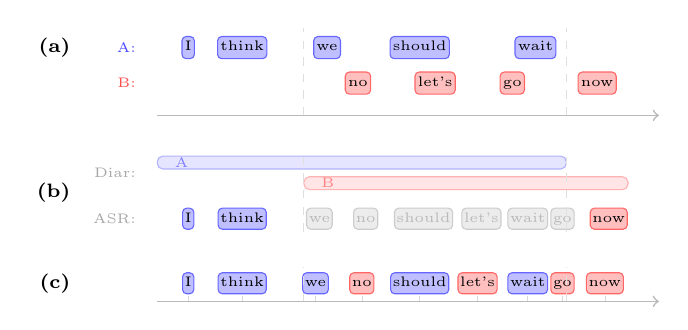
\begin{tikzpicture}[
    xscale=0.98,
    yscale=0.82,
    spkA/.style={fill=blue!25, draw=blue!60, rounded corners=1.5pt, minimum height=0.28cm, inner sep=1pt, font=\tiny\strut},
    spkB/.style={fill=red!25, draw=red!60, rounded corners=1.5pt, minimum height=0.28cm, inner sep=1pt, font=\tiny\strut},
    spkAt/.style={fill=blue!25, draw=blue!60, rounded corners=1.5pt, minimum height=0.26cm, inner sep=0.8pt, font=\tiny\strut},
    spkBt/.style={fill=red!25, draw=red!60, rounded corners=1.5pt, minimum height=0.26cm, inner sep=0.8pt, font=\tiny\strut},
    amb/.style={fill=gray!15, draw=gray!40, rounded corners=1.5pt, minimum height=0.24cm, inner sep=0.8pt, font=\tiny\strut, text=gray!55},
    timeline/.style={->, semithick, gray!55},
    lbl/.style={font=\scriptsize\bfseries, anchor=east},
]

% ---- (a) Ground truth ----
\node[lbl] at (-0.7, 2.6) {(a)};

\node[spkA] at (0.7, 2.6) {I};
\node[spkA] at (1.4, 2.6) {think};
\node[spkA] at (2.5, 2.6) {we};
\node[spkA] at (3.7, 2.6) {should};
\node[spkA] at (5.2, 2.6) {wait};

\node[spkB] at (2.9, 2.05) {no};
\node[spkB] at (3.9, 2.05) {let's};
\node[spkB] at (4.9, 2.05) {go};
\node[spkB] at (6.0, 2.05) {now};

\node[font=\tiny, blue!70, anchor=east] at (0.15, 2.6) {A:};
\node[font=\tiny, red!70, anchor=east] at (0.15, 2.05) {B:};

\draw[timeline] (0.3, 1.55) -- (6.8, 1.55);
\draw[dashed, gray!25, thin] (2.2, 1.55) -- (2.2, 2.9);
\draw[dashed, gray!25, thin] (5.6, 1.55) -- (5.6, 2.9);


% ---- (b) Cascade ----
\node[lbl] at (-0.7, 0.35) {(b)};

\draw[fill=blue!10, draw=blue!30, rounded corners=2pt] (0.3, 0.72) rectangle (5.6, 0.92);
\node[font=\tiny, blue!50, anchor=west] at (0.4, 0.82) {A};
\draw[fill=red!10, draw=red!30, rounded corners=2pt] (2.2, 0.4) rectangle (6.4, 0.6);
\node[font=\tiny, red!50, anchor=west] at (2.3, 0.5) {B};
\node[font=\tiny, gray!70, anchor=east] at (0.15, 0.66) {Diar:};

\node[font=\tiny, gray!70, anchor=east] at (0.15, -0.05) {ASR:};
\node[spkAt] at (0.7, -0.05) {I};
\node[spkAt] at (1.4, -0.05) {think};
\node[amb] at (2.4, -0.05) {we};
\node[amb] at (3.0, -0.05) {no};
\node[amb] at (3.75, -0.05) {should};
\node[amb] at (4.5, -0.05) {let's};
\node[amb] at (5.1, -0.05) {wait};
\node[amb] at (5.55, -0.05) {go};
\node[spkBt] at (6.15, -0.05) {now};

\draw[dashed, gray!25, thin] (2.2, -0.25) -- (2.2, 1.0);
\draw[dashed, gray!25, thin] (5.6, -0.25) -- (5.6, 1.0);


% ---- (c) Shuffle ----
\node[lbl] at (-0.7, -1.05) {(c)};

\node[spkAt] at (0.7, -1.05) {I};
\node[spkAt] at (1.4, -1.05) {think};
\node[spkAt] at (2.35, -1.05) {we};
\node[spkBt] at (2.95, -1.05) {no};
\node[spkAt] at (3.7, -1.05) {should};
\node[spkBt] at (4.45, -1.05) {let's};
\node[spkAt] at (5.1, -1.05) {wait};
\node[spkBt] at (5.55, -1.05) {go};
\node[spkBt] at (6.1, -1.05) {now};

\foreach \x in {0.7, 1.4, 2.35, 2.95, 3.7, 4.45, 5.1, 5.55, 6.1} {
    \draw[gray!30, very thin] (\x, -1.25) -- (\x, -1.33);
}
\draw[timeline] (0.3, -1.33) -- (6.8, -1.33);

\draw[dashed, gray!25, thin] (2.2, -1.33) -- (2.2, -0.8);
\draw[dashed, gray!25, thin] (5.6, -1.33) -- (5.6, -0.8);

\end{tikzpicture}
\caption{%
Word-level speaker attribution in overlapped speech.
\textbf{(a)}~Ground truth: speakers A (\textcolor{blue!60}{blue}) and B (\textcolor{red!60}{red}) produce concurrent tokens with partial overlap (dashed).
\textbf{(b)}~Cascade: diarization detects both speakers as active, but all ASR words in the overlap are ambiguous (gray) since both segments cover the same time.
\textbf{(c)}~Shuffle: the Viterbi path produces an interleaved, time-aligned, speaker-attributed sequence.
}
\label{fig:overlapped_attribution}
\vspace{-4mm}
\end{figure}